% --- MODELLAZIONE BLACK BOX ---

\section{Black Box Approaches}


%\subsection{Architecture*}
\begin{frame}{Black Box Approaches - Architecture}
    Standard Neural Network for setting a \textbf{baseline} for learning the double pendulum dynamics

    \begin{figure}[h]
        \centering
        \includegraphics[width=0.6\linewidth]{04_baseline_bb/DynNN.pdf} \\
        \vspace{0.3em}
    \end{figure}    %

    %The model takes as inputs the \textbf{states} and outputs the \textbf{derivatives}

    \begin{block}{Training methods}

        \begin{itemize}
            \item \textbf{Derivatives}: loss is computed directly on the derivatives
            \item \textbf{Evolution}: the derivatives are fed to a \textbf{solver} that outputs the next state. A sequential stream of predicted
            states is used to compute the loss
        \end{itemize}
    \end{block}
\end{frame}

\begin{frame}{Evolution Training}
    
    \begin{figure}[h]
        \centering
        \includegraphics[width=0.7\linewidth]{04_baseline_bb/integrator.pdf} \\
        \vspace{0.3em}
        \caption{Evolution training architecture using RK4}
    \end{figure}
     
\end{frame}

%\subsection{Training Recipe}

\begin{frame}{Black Box Approaches - Training recipe (1)}
    

    \begin{block}{Trigonometric Transformation}
        \[
            \begin{bmatrix}
                    q_1 \\
                    q_2 \\
                    \dot{q}_1 \\
                    \dot{q}_2 \\
            \end{bmatrix} \in \mathbb{R}^4
            \mapsto 
            \begin{bmatrix}
                \cos(q_1) \\
                \sin(q_1) \\
                \cos(q_2) \\
                \sin(q_2) \\
                \dot{q}_1 \\
                \dot{q}_2 \\
            \end{bmatrix}
            \in \mathbb{R}^6
        \]
    \end{block}

    \vspace{0.3cm}
    \textbf{Why do we use a TrigLayer?}
    
    \begin{itemize}
        \item \textbf{Hard-Coding Physics (Inductive Bias):} we prevent wasting the Universal Approximator's capacity on learning basic periodic functions
        \item \textbf{Intrinsic Scaling:} the angular inputs are naturally bounded within the range $[-1, 1]$
        \item \textbf{Continuity:} the transformation ensures continuity at the angle wrap-around points (e.g., $-\pi$ to $\pi$), avoiding discontinuities that may confuse the model during training
    \end{itemize}
    
\end{frame}

\begin{frame}{Black Box Approaches - Training recipe (2)}

    \begin{block}{Curriculum learning}

        Essential for \textbf{trajectory evolution} (long-term prediction)
        
        \vspace{1em}
        \textbf{Method:} start with small horizon $H$, then increase progressively
        $ H_{k+1} \leftarrow 2 \cdot H_k $
        
        \vspace{0.5em}
        \textbf{Why:} 
        \begin{itemize}
            \item prevents \alert{gradient explosion} caused by long horizons at early training stages
            \item helps the model to gradually learn long-term dependencies
        \end{itemize}
    \end{block}
    
\end{frame}

\begin{frame}{Black Box Approaches - Training recipe (3)}
    % TODO: update velocities and acceleration fitted with gaussian and laplacian respectively
    \begin{block}{Standardization}
        \begin{columns}[T]
            
            \begin{column}{0.5\textwidth}
                \centering
                \vspace{0.5em}
                \textbf{Velocities - Gaussian distribution}

                \begin{figure}[h]
                    \centering
                    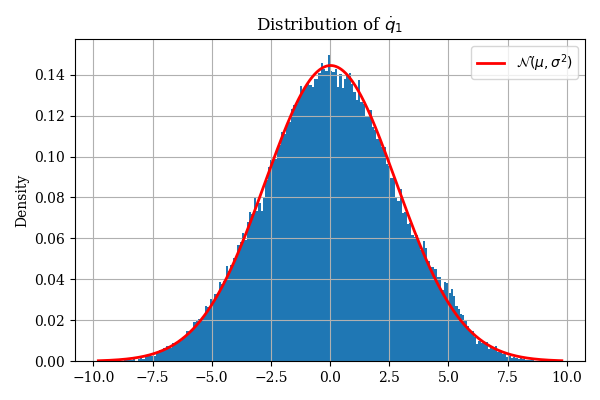
\includegraphics[width=0.8\linewidth]{Images/04_baseline_bb/Gaussian.png} \\
                    \vspace{0.3em}
                \end{figure}    

                \vspace{-3em}
        
                $$\hat{\dot{q}}_i = \frac{\dot{q_i} - \mu_{\dot{q}_i}}{\sigma_{\dot{q}_i}}$$
                $$i = 1, 2$$
            \end{column}
            
            \begin{column}{0.5\textwidth}
                \centering
                \vspace{0.5em}
                \textbf{Accelerations - Laplacian distribution}

                \begin{figure}[h]
                    \centering
                    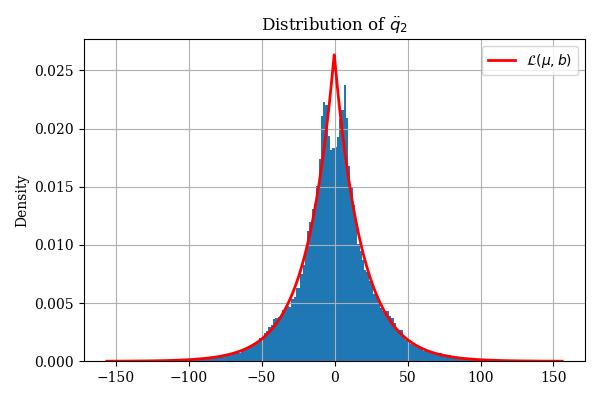
\includegraphics[width=0.8\linewidth]{Images/04_baseline_bb/Laplacian.png} \\
                    \vspace{0.3em}
                \end{figure}    
                
                \vspace{-3em}
            
                $$\hat{\ddot{q}}_i = \frac{\ddot{q}_i - \mu_{\ddot{q}_i}}{\sqrt{2b}}$$ 
                
                with $b = \mathbb{E}\bigl[|q - \tilde{\mu}|\bigr]$
                
                
            \end{column}
        \end{columns}
        
    \end{block}
\end{frame}



\begin{frame}{Black Box Approaches - Training recipe (4)}
    
    % \begin{block} {Learning rate}
    %     A learning rate scheduler is used 

    % \end{bloc

    \begin{columns}[c] %

        \begin{column}{0.35\textwidth}
            \begin{block}{Sample weights}
                Computed using the 4D KDE of the input distribution. In particular: 

                % TODO: update max or total
                $$\sigma(q_1, q_2, \dot{q}_1, \dot{q}_2) = $$
                $$ = \frac{h_{tot}}{h(q_1, q_2, \dot{q}_1, \dot{q}_2)}$$
                then normalized such that $\sum \sigma_i = 1$

                Important: multivariate distribution capture any \textbf{coupling term} in the dynamics
            \end{block}
        \end{column}
        
        \begin{column}{0.6\textwidth} 
            \centering
            \includegraphics[width=0.85\linewidth]{04_baseline_bb/sample_weights.png}
        \end{column}
    
        

    \end{columns}

    


\end{frame}



%\subsection{Results}

\begin{frame}{Black Box Approaches - Results (1)}
    
    \begin{figure}[h]
            \centering
            \includegraphics[width=0.8\linewidth]{04_baseline_bb/deep_ez.png} \\
    \end{figure}   
        
     

\end{frame}


\begin{frame}{Black Box Approaches - Results (2)}

     \begin{figure}[T]
        \centering
        \includegraphics[width=0.8\linewidth]{04_baseline_bb/Deep_hard.png} \\
    \end{figure} 
    
     

\end{frame}



\begin{frame}{Black Box Approaches - Energy drift}
    \centering Energy evolution over time with \textbf{no friction}
    \textbf{}
    
    \begin{figure}[T]
        \centering
        \includegraphics[width=0.8\linewidth]{04_baseline_bb/energy_drift.png} \\
    \end{figure}

    The system is \textbf{not able to conserve energy}. 

\end{frame}




